\chapter{Background}
\label{ch:Background}
In this chapter the fundamentals to understand the methods used in this thesis are explained.
The first section gives some mathematical background for different ways to represent orientations.
In \cref{sec:sensors} the functionality of the different sensors used in this thesis are explained.
A brief overview of the field of computer vision is given in \cref{sec:computer_vision}.
Lastly, in \cref{sec:ros} the \gls{ros} framework, which allows for the communication to the different sensors, is introduced.


\section{Mathematical Background}
\subsection{Mathematical Representations of 3D Orientations}
Different sensors will be used in this thesis and each sensor will make its measurements in its own coordinate frame.
In order to obtain meaningful results, all frames must be aligned to one common frame.
The necessary 3D rotations can be expressed in several ways, I will briefly describe the ones used in this thesis.

\subsubsection{Rotation Matrix}
A rotation matrix \mtf{b}{a} $\in \mathbb{R}^{3\times3}$ transforms an arbitrary vector from the coordinate system $\mathcal{B}$ to the coordinate system $\mathcal{A}$.
Rotation matrices have the following properties
\begin{equation}
	\mathbf{M}\mathbf{M}^\intercal = \mathbf{M}^\intercal \mathbf{M} = I_3, \quad \det \mathbf{M} = 1.
\end{equation}
The rows of the rotation matrix are the axes of the new coordinate system.
A rotation matrix corresponds to two different rotations, but uniquely describes an orientation.
Rotation matrices can be concatenated, but this must be done in reverse order, e.g.
\begin{equation}
	{}_\mathcal{C}\vb{p} = \mtf{a}{c}{}_\mathcal{A}\vb{p} = \mtf{b}{c}\mtf{a}{b}{}_\mathcal{A}\vb{p}
\end{equation}
to transform the point ${}_\mathcal{A}\vb{p}$ over the intermediate frame $\mathcal{B}$ to the coordinate system $\mathcal{C}$.

\subsubsection{Euler Angles}
Euler angles are the closest to intuition but mathematically the worst way to represent orientations.
Every orientation can be produced by a concatenation of three rotations around each of the coordinate axes.
Because the resulting orientation depends on the order of which the rotations were performed, there are different conventions.
Furthermore, the conventions can be divided into intrinsic and extrinsic.
Intrinsic rotation means that the coordinate system moves with the moving object, whereas with extrinsic rotations the original coordinate system remains static.\\
The most common convention is the zyx (intrinsic), which first rotates an angle $\psi$ around the z-axis, followed by a rotation of $\theta$ around the y-axis and finally an angle $\phi$ around the x-axis, see \cref{fig:tikz_euler_angles}.
\begin{figure}[htpb]
	\centering
	\documentclass{standalone}
\usepackage{tikz}
\usepackage{tikz-3dplot}

\begin{document}
% Set the plot display orientation
% Syntax: \tdplotsetdisplay{\theta_d}{\phi_d}
\tdplotsetmaincoords{60}{110}

% Start tikz-picture, and use the tdplot_main_coords style to implement the display
% coordinate transformation provided by 3dplot.
\begin{tikzpicture}[scale=3,tdplot_main_coords]

    % Set origin of main (body) coordinate system
    \coordinate (O) at (0,0,0);

    % Draw main coordinate system
    \draw[black, thick,->] (0,0,0) -- (1,0,0) node[anchor=north east]{$x$};
    \draw[black, thick,->] (0,0,0) -- (0,1,0) node[anchor=north west]{$y$};
    \draw[black, thick,->] (0,0,0) -- (0,0,1) node[anchor=south]{$z$};

    %Draw the arcs on each theta plane
    %The first position is obvious since we are in the x-y plane and rotating around the z-axis.
    %The anchor already went crazy, north is pointing downwards...
    \tdplotdrawarc[->,color=red]{(0,0,0.7)}{0.1}{0}{350}{anchor=south west,color=red}{$\psi$ (I)}
    %We move to the z-x axis
    \tdplotsetthetaplanecoords{0}
    %Notice you have to tell tiks-3dplot you are now in rotated coords
    %Since tikz-3dplot swaps the planes in tdplotsetthetaplanecoords, the former y axis is now the z axis.
    \tdplotdrawarc[tdplot_rotated_coords,->,color=blue]{(0,0,0.7)}{0.1}{110}{460}{anchor=south west,color=blue}{$\theta$ (II)}
    \tdplotsetthetaplanecoords{-90}
    %Once again we swaps the planes. I don't know why it's working like this but we turn backwards
    %so the arrow turns in the positive direction.
    \tdplotdrawarc[tdplot_rotated_coords,->,color=green]{(0,0,0.7)}{0.1}{120}{470}{anchor=south west,color=green}{$\phi$ (III)}
    % If you turn the theta plane  of 90 degrees position and rotation are inverted.
    %\tdplotsetthetaplanecoords{90}
    %\tdplotdrawarc[tdplot_rotated_coords,->,color=black]{(0,0,-0.7)}{0.1}{470}{120}{anchor=south east,color=black}{roll}
\end{tikzpicture}

\end{document}
	\caption[zxy Euler convention]{Definition of the zyx Euler convention. The rotation starts with a rotation $\psi$ around the z-axis and ends with a rotation $\phi$ around the x-axis.}
	\label{fig:tikz_euler_angles}
\end{figure}

The angles are called yaw (or heading), pitch and roll respectively. Roll and pitch angle together are also often referred to as inclination.\\
The disadvantages of Euler angles are the many conventions and the possibility of singularity.
Unlike rotation matrices, Euler angles do not uniquely describe a rotation.
Singularity, which is also referred to as gimbal lock when occurring in mechanical gyroscopes, occurs when the pitch angle is set to $\theta = \frac{\pi}{2}$.
The other two angles are then undefined, because both their rotations axes are parallel to each other \cite{Kok2017}.

\subsubsection{Quaternions}
A quaternion is defined as
\begin{equation}
	\vb{q} = q_w + q_x\vb{i} + q_y\vb{j} + q_z\vb{k}
\end{equation}
with a real part $q_w$ and three imaginary parts $\vb{i}, \vb{j}$ and $\vb{k}$ satisfying
\begin{equation}
	\vb{i}^2 = \vb{j}^2 = \vb{k}^2 = \vb{i}\vb{j}\vb{k} = -1.
\end{equation}
The quaternion can also be written in vector form by dividing the quaternion in a real or scalar part $q_w$ and an imaginary or vector part $q_v = \begin{pmatrix} q_x & q_y & q_z	\end{pmatrix}^\intercal$
\begin{equation}
	\vb{q} = \begin{pmatrix}
		\vb{q}_v \\
		q_w
	\end{pmatrix}
	=\begin{pmatrix}
		q_x & q_y & q_z & q_w
	\end{pmatrix}^\intercal.
\end{equation}
Note that in some literature the order of the real and imaginary part are swapped.
If the quaternion is a unit vector, which means it satisfies
\begin{equation}
	\abs*{\vb{q}} = \sqrt{\vb{q}^\intercal \vb{q}} = \sqrt{\abs*{\vb{q}_v^2 + q_w^2}} = 1
\end{equation}
then it can be used to represent rotations.
The rotation is then described with
\begin{equation}
	\label{eq:quaternion}
	\vb{q} =
	\begin{pmatrix}
		\hat{\vb{j}}\vdot\sin(\frac{\alpha}{2}) \\
		\cos(\frac{\alpha}{2})
	\end{pmatrix}
\end{equation}
with $\alpha$ being the rotation angle and $\hat{\vb{j}}$ being the normalized rotation axis.
Each rotation is uniquely described by one unit quaternion, but each orientation can be described by two unit quaternions with opposite signs.
A rotation to transform a point ${}_\mathcal{A}\vb{p}$ from frame $\mathcal{A}$ to $\mathcal{B}$ is defined as
\begin{equation}
	{}_\mathcal{B}\vb{p} = \qtf{a}{b} \otimes {}_\mathcal{A}\overline{\vb{p}} \otimes \qtf{a}{b}^*,
\end{equation}
where
\begin{equation}
	{}_\mathcal{A}\overline{\vb{p}} = \begin{pmatrix}
		0 & {}_\mathcal{A}\vb{p}^\intercal
	\end{pmatrix}^\intercal,
\end{equation}
and $\qtf{a}{b}^* = \qtf{b}{a}$ is the conjugate defined as
\begin{equation}
	\qtf{}{}^* = \begin{pmatrix}
		-\vb{q}_v \\
		q_w
	\end{pmatrix}.
\end{equation}
The symbol $\otimes$ denotes the quaternion multiplication, which is given by
\begin{equation}
	\vb{p} \otimes \vb{q} =
	\begin{pmatrix}
		p_{w} q_{w}-p_v \cdot q_v \\
		p_{w} q_v+q_{w} p_v+p_v \times q_v
	\end{pmatrix}.
\end{equation}
A quaternion can be converted to a rotation matrix with
\begin{equation}
	\label{eq:q_to_M}
	\mathbf{M} =
	\begin{pmatrix}
		1 - 2q_y^2-2 q_z^2   & 2(q_x q_y- q_z q_w) & 2(q_x q_z + q_y q_w) \\
		2(q_x q_y + q_z q_w) & 1-2 q_x^2-2 q_z^2   & 2(q_y q_z -q_x q_w)  \\
		2(q_x q_z-q_y q_w)   & 2(q_y q_z+ q_x q_w) & 1 - 2 q_x^2- 2 q_y^2
	\end{pmatrix}.
\end{equation}
More information about quaternions can be found in \cite{Kok2017,Trawny2005}.\\

\subsection{Vector Projection}
\label{subsec:vector_projection}
Vector projection is used later in this thesis to align different coordinate frames, this section describes the theory behind it.
In general, the rotation to align a vector $\vb{v}_1$ with a vector $\vb{v}_2$ can be expressed using a quaternion.
At first both vectors must be normalized, resulting in the two unit vectors $\vu{v}_1$ and $\vu{v}_2$.
The rotation axis is perpendicular to both vectors and can thus be calculated using the cross product, which is then divided by the norm, to get a unit vector
\begin{equation}
	\vb{j} = \frac{\vu{v}_1 \cp \vu{v}_2}{\norm{\vu{v}_1 \cp \vu{v}_2}}.
\end{equation}
The angle between two vectors can be calculated by
\begin{equation}
	\cos(\alpha) = \frac{\vu{v}_1 \vdot \vu{v}_2}{\norm{\vu{v}_1} \cdot \norm{\vu{v}_2}}
	= \vu{v}_1 \vdot \vu{v}_2 \implies
	\alpha = \arccos(\vu{v}_1 \vdot \vu{v}_2).
\end{equation}
The denominator is equal to 1 (because the norm of a unit vector is 1) and thus omitted.
Using \cref{eq:quaternion} the rotation can then be expressed as a quaternion.



\section{Sensors}
\label{sec:sensors}
Sensors are necessary to acquire information about the environment.
In this section the functionality and advantages and disadvantages of each sensor used in this thesis will be described.

\subsection{\glsentryfull{imu}}
An \gls{imu} is used to track the orientation and position of an object.
Common uses are in the aerospace or automotive industry, often in combination with other sensors, to give information about the pose and position of a vehicle.
More recently with the invention of \gls{mems} and specifically \gls{mems}-\glspl{imu} which allow for a very small form factor at a low cost, \glspl{imu} are also used in consumer electronics such as smartphones or fitness tracker.
An \gls{imu} usually consists of the three following sensors.\\
The acceleration is measured using an accelerometer and can be used to determine the velocity and the covered distance by integrating the acceleration with respect to time once respectively twice.
The gyroscope gives information about the change of orientation.
The third part is the magnetometer, which is able to measure the earth's magnetic field and is used to correct the measurements of the gyroscope.
It allows for the determination of the absolute heading, whereas the gyroscope can only measure relative change. But because it is very sensitive to other magnetic objects, it is often omitted.
\glspl{imu} can be typically divided into the two following categories.
\begin{figure}[h]
	\centering
	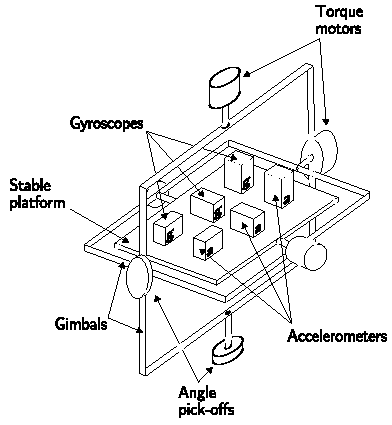
\includegraphics[width=0.4\linewidth]{stable_platform_imu}
	\caption[Setup of a stable platform \acrshort{imu}]{Setup of a stable platform \acrshort{imu} \cite{Woodman2007}.}
	\label{fig:stable_platform_imu}
\end{figure}
\\In the first type, the stable platform systems, the inertial sensors are mounted in such way, that they are always aligned with the reference frame.
This is achieved using gimbals, which allow movement along all three axes.
The gyroscopes on the platform measure the rotation and send them to torque motors, which rotate the gimbals to keep the platform in alignment with the reference frame.
A typical setup of a stable platform system can be seen in \cref{fig:stable_platform_imu}.
The advantage of a stable platform systems is that the calculation of orientation and position is straightforward.
The angles of the gimbals can be measured to receive the orientation and position, the accelerometer measurements have to be corrected for gravity and be integrated two times.
No coordinate transformation is necessary.
The disadvantages are that the mechanical structure of the setup is complex, needs regular maintenance, requires a lot of space and has high costs.\\
The second type are strap down systems, which are mostly used today.
As the name suggests all the parts are fixed onto the device and are thus not anymore always aligned with the reference frame.
Advantages are that due to the lack of gimbals and motors a significantly smaller build is possible while also being cheaper to mass produce.
A disadvantage is that the calculation of the orientation and position is more complex, the rate gyroscopes have to be integrated to get the orientation and can then be used to transform the accelerometer signals into the reference frame.
But with the decrease of computational cost this disadvantages continues to diminish.\\
There are many types of gyroscopes and accelerometers such as mechanical, optical or solid state, but only the functionality of \gls{mems} will be described, because those will also be used in the experiment.
Information about the working principle of other systems and also much more information about \glspl{imu} in general can be found in \cite{Woodman2007}.\\
\gls{mems} consist of electrical and/or mechanical components in the size of \SI{100}{\nano\metre} to \SI{1}{\milli\metre}, allowing for a very small form factor.
Other characteristics of \gls{mems} are that they can easily be mass-produced allowing for low cost and usually also need less power than traditional systems, because everything is integrated on the chip \cite{Shaeffer2013}.
Almost all consumer grade electronics uses \gls{mems}-\glspl{imu} nowadays, but they also find more and more use in many industry segments, as their accuracy continues to improve \cite{Perlmutter2016}.

\subsubsection{\glsentryshort{mems} Accelerometer}
\begin{figure}[htb]
	\centering
	\begin{subfigure}{0.48\textwidth}
		\centering
		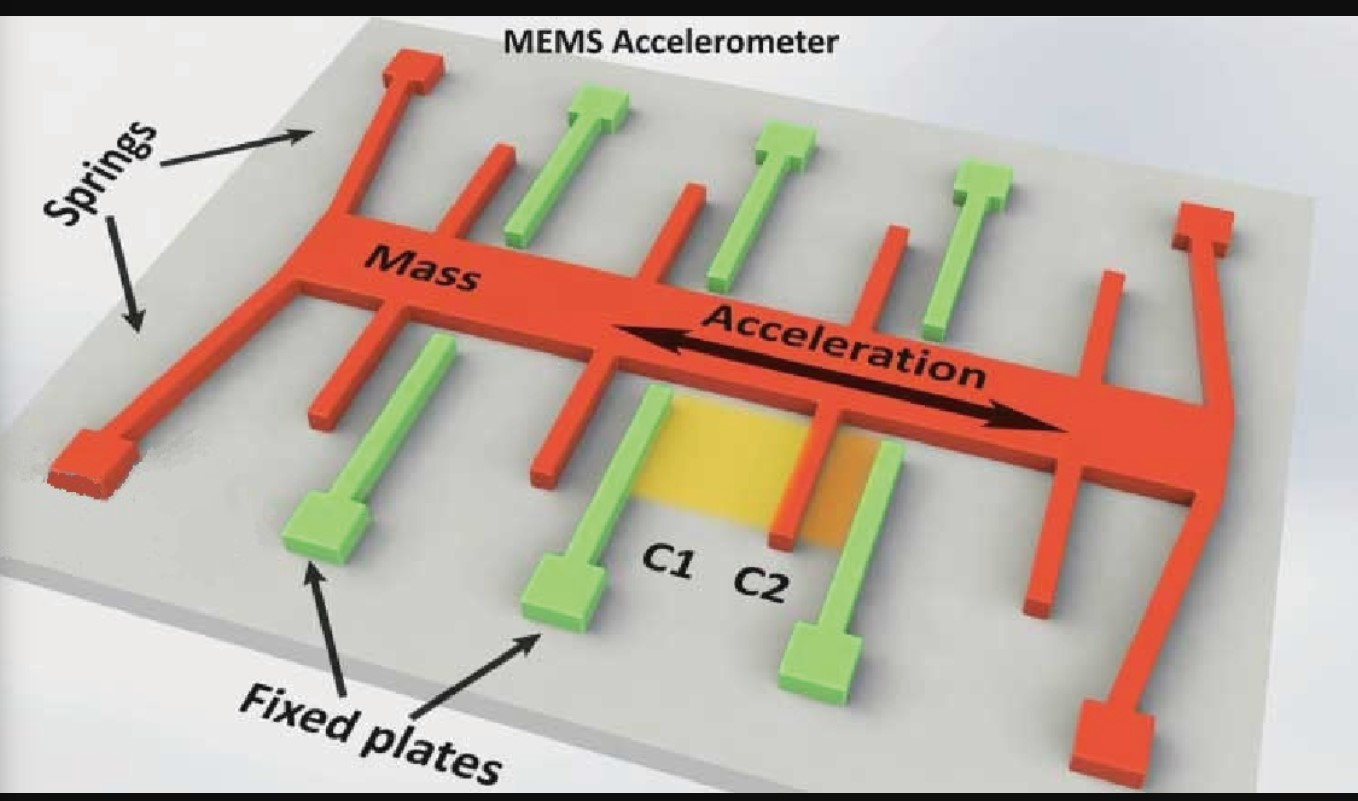
\includegraphics[width=\textwidth]{MEMS_Accelerometer}
		\caption{\acrshort{mems} accelerometer}
		\label{fig:MEMS_Accelerometer}
	\end{subfigure}
	% \hfill
	\begin{subfigure}{0.48\textwidth}
		\centering
		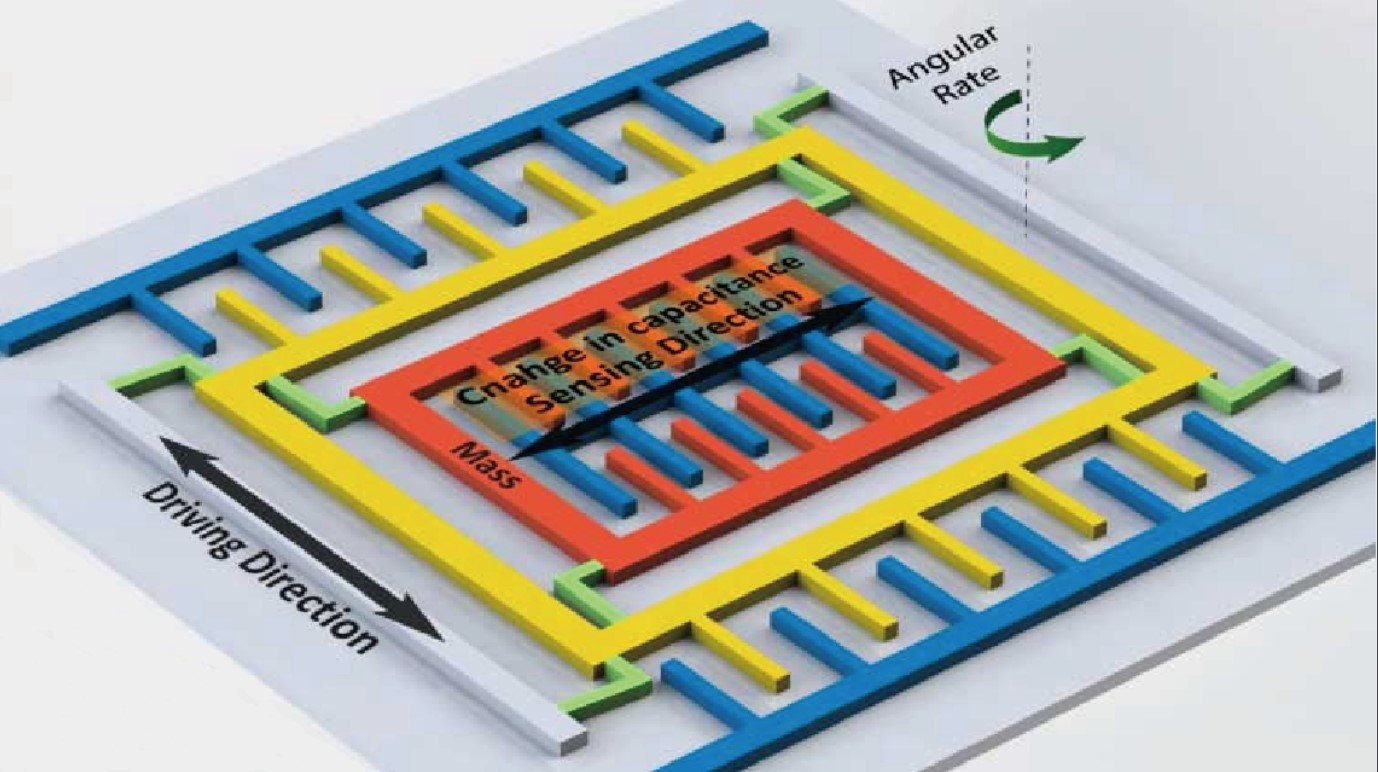
\includegraphics[width=\textwidth]{MEMS_Gyroscope}
		\caption{\acrshort{mems} gyroscope}
		\label{fig:MEMS_Gyroscope}
	\end{subfigure}
	\caption[Micro structure of a \acrshort{mems} accelerometer and gyroscope]{Micro structure of a \acrshort{mems} accelerometer and gyroscope. \color{red}TODO: Better images (with ref or make own)}
	\label{fig:MEMS_design}
\end{figure}
The accelerometer is used to measure the acceleration.
Additional to the dynamic acceleration there is the static and constant gravity acceleration on earth, which is measured by the \gls{imu} in upward direction.
This allows for the determination of one axis of the \gls{imu}, even if it is not moving.
Often times only the dynamic accelerations are of interest and to get them the acceleration data during stand still must be measured and subtracted.\\
The microstructure of a \gls{mems} accelerometer is shown in \cref{fig:MEMS_Accelerometer}.
A mass is suspended by springs along one axis and if an acceleration along this axis occurs, the mass moves in the opposite direction due to Newton's second law.
The mass has little fingers perpendicular to the axis along which the movement occurs, which affect the capacity between the fixed plates.
The change of capacity and thus voltage can be measured, from which the acceleration can be calculated.
To be able to measure the acceleration along all three axis the same setup is used three times, perpendicular to each other.\\
The accelerations $\hat{\vb{a}}$ measured with a \gls{mems} accelerometer are not free of noise and can be modeled according to \cite{Lefferts1982} in a simplified way as
\begin{equation}
	\hat{\vb{a}} = \vb{a} + \vb{b}_\mathrm{a} + \vb{n}_\mathrm{a}.
\end{equation}
The measurement differs from the true acceleration $\vb{a}$ due to random noise $\vb{n}_\mathrm{a}$ and a slowly time-varying bias $\vb{b}_\mathrm{a}$.
More about the specific error terms can be read in \cref{sse:mems_errors}.

\subsubsection{\glsentryshort{mems} Gyroscopes}
A gyroscope measures the angular velocity.
The setup of a \gls{mems} gyroscope is similar to that of a \gls{mems} accelerometer.
A proof mass is suspended on a frame and responds to an input force.
\gls{mems} gyroscopes make use of the Coriolis effect, which states that a rotating object with the angular velocity $\boldsymbol{\omega}$ of mass $m$ and velocity $\vb{v}$ experiences a force
\begin{equation}
	\vb{F}_\mathrm{C}  = -2m(\boldsymbol{\omega}\times \vb{v}).
\end{equation}
To measure the effect, a mass is vibrating along one axis, which in turn is also suspended.
If the mass is oscillating along one axis and a rotation is applied, a second oscillation on the axis perpendicular to the rotation axis can be observed.
E.g.\ if the mass oscillates along the x-axis and a rotation around the z-axis is applied, a vibration along the y-axis can be observed.
By measuring the amplitude and phase of the secondary oscillation the absolute value and direction of the angular velocity can be calculated.
While \gls{mems} gyroscopes do not achieve the same accuracy as optical gyroscopes they offer many advantages such as smaller physical properties (weight and size), lower power consumption and startup time as well as a significantly lower cost.
\gls{mems} gyroscopes have replaced other gyroscope types in most areas, but in areas where the highest precision possible is necessary, typically in military industry, optical gyroscopes are still used today \cite{Perlmutter2016}.\\
Similar to the accelerometer, the measurements $\hat{\boldsymbol{\omega}}$ of the \gls{mems} gyroscope are influenced by errors, which can be modeled according to \cite{Lefferts1982} as
\begin{equation}
	\hat{\boldsymbol{\omega}} = \boldsymbol{\omega} + \vb{b}_\mathrm{g} + \vb{n}_\mathrm{g}.
\end{equation}
The measurement differs from the true angular velocity $\boldsymbol{\omega}$ due to the slowly time-varying bias vector $\vb{b}_\mathrm{g}$ and the random noise vector $\vb{n}_\mathrm{g}$, which has a mean of zero.

\subsubsection{(\glsentryshort{mems}) Magnetometer}
A magnetometer measures the local magnetic field.
Most sensors work using the Hall effect.
A current is set to flow through a conductive plate.
Without the presence of a magnetic field the electrons flow in a straight line, but if a magnetic field is introduced the electrons do get deflected to one side.
The voltage between the two sides can then be measured, from which the strength and direction of the magnetic field can be determined.\\
Without any magnetic disturbances, the magnetometer measures a constant local magnetic field vector.
The vector points to magnetic North and can thus be used to determine the heading.
Because the magnitude of the earth's magnetic field is very low (\SIrange{25}{65}{\micro\tesla}), the magnetometer readings can easily be influenced by other objects \cite{Kok2016}.\\
The distortions can be divided into two categories: hard or soft iron.
Hard iron distortions are created by objects which actively produce a magnetic field, causing a permanent bias.
Soft iron disturbances are due to deflections or altercations of an existing magnetic field.
Both types of disturbances can be removed with a proper calibration if their position and orientation, relative to the sensor, stays the same \cite{Guo2008}.
Every time the sensor is placed in a (magnetically) new environment, a recalibration is necessary.

\subsubsection{Typical \glsentryshort{mems} Errors}
\label{sse:mems_errors}
The errors can be divided into two categories: systematic and stochastic errors \cite{Zhang2019}.\\
Systematic errors or also known as calibration errors are constant over time and can be eliminated by calibration.
Typical examples are bias (offset), scaling or axis misalignment.
Integrating a constant bias once or twice leads to a drift (error grows linearly with respect to time) or a second-order drift (error grows quadratically) respectively.
Hence, the elimination of the bias is necessary to get reliable estimations of the orientation, velocity or position, which are calculated by integrating the angular velocity or the accelerometer measurements.\\
Stochastic errors change at every measurement and can be modeled using a statistical approach.
The turn-on bias is different every time the \gls{imu} is powered up, but can be eliminated after a rest period.
Errors due to temperature fluctuations influencing the measurements are also common, but because most \glspl{imu} are equipped with a temperature sensor, the introduced error can be eliminated.
Harder to correct is the introduced error due to thermo-mechanical noise, which is measured as white noise.
The integration of white noise leads than to a random walk.\\
Angle errors introduced by random walk are usually the hardest to correct and are the reason, why the measurements of the gyroscope can not be trusted over a long period of time \cite{Woodman2007}.


\subsection{\glsentryfull{lidar}}
\gls{lidar} is a method to measure distance to objects.
Similar to other systems such as \gls{sonar} or \gls{radar}, \gls{lidar} uses the time-of-flight principle.
A short laser pulse with the velocity of light $c$ is sent into the environment and the reflected light is analyzed.
The duration $\Delta t$ it took from sending to receiving can then be used to calculate the distance $s$ between the \gls{lidar} and the object that the light hit with
\begin{equation}
	s = c\frac{\Delta t}{2}.
\end{equation}
The change of intensity and wavelength of the returning light are measured as well and can provide information about the reflectivity of the object (intensity) or the chemical composition of the air (wavelength).
Common uses of \gls{lidar} are the analysis of earth's atmosphere, 3D mapping of environments or in the field of autonomous driving for object detection, tracking and \gls{slam}.
Basically all applications which use \gls{radar} can also be used with a \gls{lidar} instead, allowing for a greater accuracy.\\
There are different \gls{lidar} types, but their working principles are similar.
A transmitter generates a signal and sends it into the environment using a scanning system and a transmission optic.
As transmitter a laser with a wavelength of \SIrange{850}{950}{\nano\metre} (near-infrared) is typically used.
The scanning system allows the laser to explore a large area instead of only a single point by steering the light at different azimuths and vertical angles and can be divided in mechanical spinning or solid state systems.
Mechanical spinning systems is the oldest technology and is still mainly used today.
A mirror which can be rotated around an axis is used, allowing for a greater vertical \gls{fov}.
Moreover, the whole \gls{lidar} base on which the laser is mounted can be rotated independently from the mirror, allowing for a \SI{360}{\degree} horizontal \gls{fov}.
To get a sufficient resolution the \gls{lidar} has to spin at a high speed, but some \glspl{lidar} also use additionally a vertical array of lasers instead of only one, to further increase the density of the generated point cloud.
The working principle of a \gls{lidar} using the mechanical spinning method is shown in \cref{fig:lidar}.
\begin{figure}[htb]
	\centering
	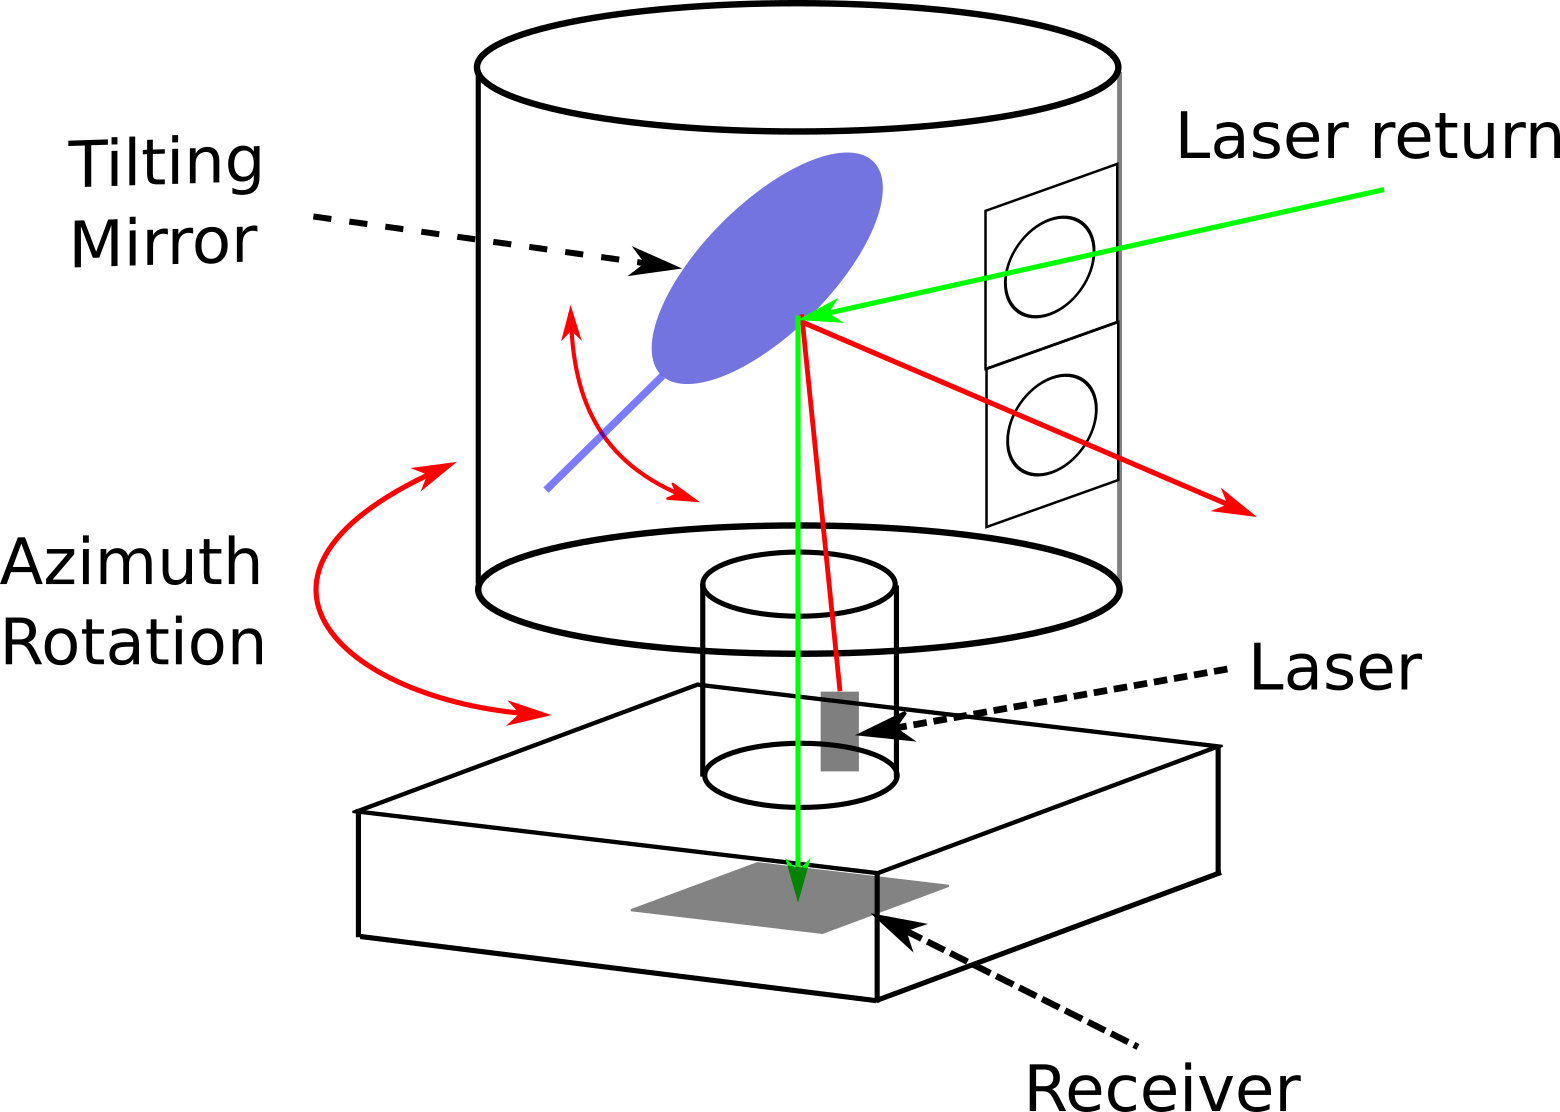
\includegraphics[width=0.5\textwidth]{Lidar.png}
	\caption[Setup of a mechanical spinning \acrshort{lidar}]{Setup of a mechanical spinning \acrshort{lidar} \cite{Li2020}. The laser is reflected off a tilting mirror and is received through a transmission optic by the receiver. A rotation of the base independently of the mirror allows for a \SI{360}{\degree} horizontal \gls{fov}.}
	\label{fig:lidar}
\end{figure}
While mechanical spinning systems are very precise and offer a great \gls{fov}, they are bulky, need a lot of power and are expensive \cite{Fujii2005}.\\
Solid state systems and especially \gls{mems} \glspl{lidar} try to overcome those problems.
\gls{mems}-\gls{lidar} are quasi-static, the only part that moves is the on the chip embedded mirror, but because of the small size (\SIrange{1}{7}{\milli\metre} diameter), very little power has to be used to move it.
The mirror can be rotated on up to two axes, but because the base cannot be rotated as with mechanical systems, a horizontal view of \SI{360}{\degree} is not possible.
Though by using multiple lasers with different incident angles the \gls{fov} can be increased.
Advantages of \gls{mems}-\glspl{lidar} compared to mechanical systems are the smaller form factor and lower cost \cite{Wang2020}.\\
After transmitting the laser signal the reflected light passes through the receiving optic and is received by photodetectors.
A processing unit then generates a 3D point cloud from all the received measurements.


\subsection{Wheel Speed Sensor}
The wheel speed sensors measure the speed of each wheel and allow for the calculation of the car velocity.
The measurements are also used by many driver assistance systems such as \gls{abs} to be able to detect wheel slip.
Different techniques exist to measure the speed with the most common ones being magnetoelectric and Hall type wheel speed sensors.
\begin{figure}[htb]
	\centering
	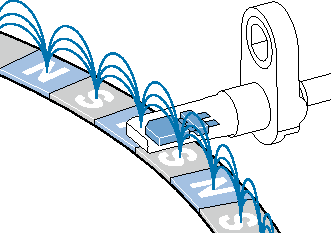
\includegraphics[width=0.5\linewidth]{wheel_speed_sensor_active.pdf}
	\caption[Setup of an active wheel speed sensor]{Setup of an active wheel speed sensor \cite{Re2011}. The sensor head measures the alternating magnetic field. The amplitude of the induced voltage can then be used to determine the wheel speed.}
	\label{fig:wheel_speed_sensor_active}
\end{figure}
\\The magnetoelectric sensor is composed of a sensor head and a ring gear.
The head is mounted stationary on the car frame while the ring gear is mounted on the wheel hub or axle and rotates with the wheel.
The sensor head is composed of a permanent magnet core and a coil.
When the wheel and thus the ring gear turns the teeth and gaps of the wheel pass by the sensor head and change the magnetic field which induces an alternating voltage in the coil.
The amplitude and frequency of the induced voltage increases with increasing wheel speed.
Advantages of the technique are the low cost, robustness and good performance even in the presence of mud etc.
A disadvantage is the frequency dependency, very low speeds can not be measured due to the induced voltage being too small, while at very high speeds the changes can not be picked anymore up by the head \cite{AutoReif2014}.\\
Nowadays, almost exclusively the hall wheel speed sensor is used.
The functionality is similar to that of the magnetoelectric sensor, but instead of a ring gear, a ring, on which alternating north and south magnets are placed, is used.
The hall element in the sensor head measures the alternating magnetic field.
A signal amplifier and processing unit is integrated in the sensor head and thus allows for a greater detection rate and range \cite{Re2011}.
The setup is shown in \cref{fig:wheel_speed_sensor_active}.
Due to the embedded processing unit the hall wheel speed sensor is also often called an active sensor, while the magnetoelectric sensor is referred to as passive sensor.



\section{Computer Vision}
\label{sec:computer_vision}
This section gives an overview of computer vision techniques and their applications.
In this thesis a trained neural network is used to detect objects in images.
The basics of object detection and image segmentation are explained.
Furthermore, the framework of the neural network used for the training and its predecessors are discussed.
Most of the following information is from ref. \cite{Szeliski2022}, which gives a great overview over the field of computer vision.


\subsection{Object Detection}
Objection detection is a common task in the field of computer vision and is used to detect, localize and classify objects in images or videos.
In contrast to image classification, which only assigns a label to an image, objection detection allows for the detection of multiple objects by drawing a bounding box around each individual object.\\
Object detection can be divided into machine learning-based methods and deep learning-based methods.
In the traditional machine learning-based methods, features from the image must be chosen manually.
This process is very time-consuming and tedious, that is why nowadays almost exclusively deep learning-based approaches based on \gls{cnn} are used.
Here, the features are extracted automatically.


\subsection{Image Segmentation}
Image segmentation partitions an image into multiple segments or objects.
It can be divided into the three categories semantic segmentation, instance segmentation or panoptic segmentation \cite{Minaee2021}.\\
In semantic segmentation all pixels corresponding to the same class are clustered together and assigned a label.
Multiple different classes can be detected, but no difference is made between multiple instances of the same class.
Every pixel is associated with a class.\\
Instance segmentation goes one step further by also differentiating between different individual objects of the same class.
It combines objection detection, objection localization and object classification.
However, it does not classify every pixel anymore, things that are hard to enumerate such as walls and roads are ignored.\\
The panoptic segmentation combines both methods.


\subsection{Neural Networks}
An \gls{ann} is a way for a computer to detect patterns and is inspired by the biological neural networks found in animal brains.
It is based on a collection of neurons which are connected with each other.
In the input layer each neuron receives a signal, processes it and then sends a signal to its connected neurons.
Each neuron has an associated weight and threshold (also known as bias), which determines the activation of the neuron.
If the threshold has not been reached, the neuron does not fire.
The output of each neuron is calculated by a non-linear function.

\subsubsection{\glsentrylong{cnn} (\glsentryshort{cnn})}
A \gls{cnn} is a class of \gls{ann} and is usually used in the field of computer vision.
It consists of three different type of layers, convolutional, pooling and the fully connected layers.
The convolutional layers help to abstract the input image as a feature map using a filter or kernel.
Using overlapping blocks of pixels, each region of the image is scanned.
Each block is then assigned a value based on the filter.
The pooling layers reduce the complexity by pooling all pixels of a feature map together.
Redundant information is removed in this step, which reduces the calculation time, storage requirement and also reduces the risk of overfitting.
The last layer is the fully connected layer.
In the previous layers neurons of the same layer were independent of each other, whereas in this final layer all neurons are connected to each other.
In this layer the actual classification is done.
While a \gls{cnn} provides great improvement, in more complex situations with multiple objects in an image the \gls{cnn} architecture is not ideal.

\subsubsection{\glsentrylong{rcnn} (\glsentryshort{rcnn})}
\label{sssec:rcnn}
That is why in 2014 a deep convolutional network called \gls{rcnn} has been introduced \cite{Girshick2014}, which can detect up to 80 different type of objects in images.
\gls{rcnn} is a type of machine learning model designed for computer vision tasks, specifically for object detection.
It sets bounding boxes across the object regions and then applies convolutional networks independently on all the \glspl{roi}.
The working principle is shown in \cref{fig:rcnn}.
In the first step the image is divided into approximately 2000 region proposals using the selective search algorithm.
The selective search algorithm groups similar regions based on their color, texture, size and shape compatibility.
After extracting a feature vector from each region proposal a pretrained \gls{svm} algorithm is applied to each region and classifies the proposal either to the background or to one of the object classes.
Disadvantages of \gls{rcnn} are that the training of the network requires a lot of storage, and it is not possible to run \gls{rcnn} in real time.
\begin{figure}[htbp]
	\centering
	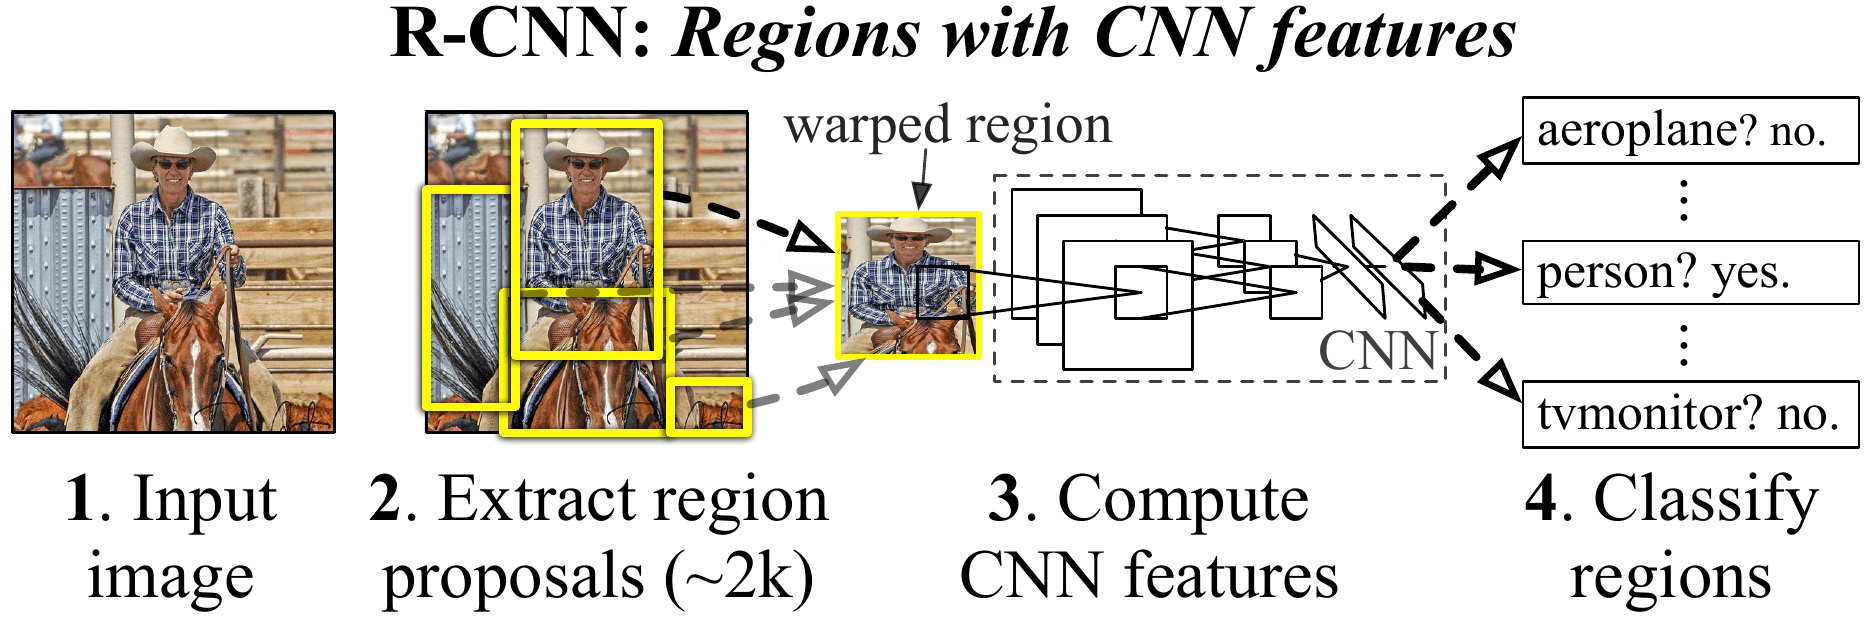
\includegraphics[width=.7\linewidth]{rcnn.png}
	\caption[\acrshort{rcnn} framework]{The \acrshort{rcnn} framework \cite{Girshick2014}. The image is divided into subregions and each subregion is classified as one of the object classes or the background independently.}
	\label{fig:rcnn}
\end{figure}
There exist multiple improvement methods with Fast \gls{rcnn} \cite{Girshick2015} and Faster \gls{rcnn} \cite{Ren2017}.
Fast \gls{rcnn} greatly improves the performance by using a new \gls{roi} pooling layer, which allows sharing computations across all proposals instead of doing it for each proposal individually.
Furthermore, it reduces the necessary storage for training the network while also providing better results.
Faster \gls{rcnn} improves the performance even further.
It uses a \gls{rpn} instead of the selective search algorithm to generate region proposals.
Advantages of \gls{rpn} over the selective search algorithm are that the network can be specifically trained and customized for the detection task.
And by using the same convolutional layers for the \gls{rpn} and the Fast \gls{rcnn} detection network, the region proposal does not take any extra time.\\
Mask \gls{rcnn} \cite{He2017} is an extension of Faster \gls{rcnn} and is a form of instance segmentation, which combines objection detection and semantic segmentation.
It adds a third branch to the Faster \gls{rcnn}, by also returning an object mask in addition to the bounding box and class label.
The process can be seen in \cref{fig:mask_rcnn}.
In the first stage \glspl{roi} are selected using a \gls{rpn}, just as with the Faster \gls{rcnn}.
The network has only to be run once on the image.
But in the second stage, a binary mask is predicted for each \gls{roi} in parallel to predicting the class and bounding box.
\begin{figure}[htbp]
	\centering
	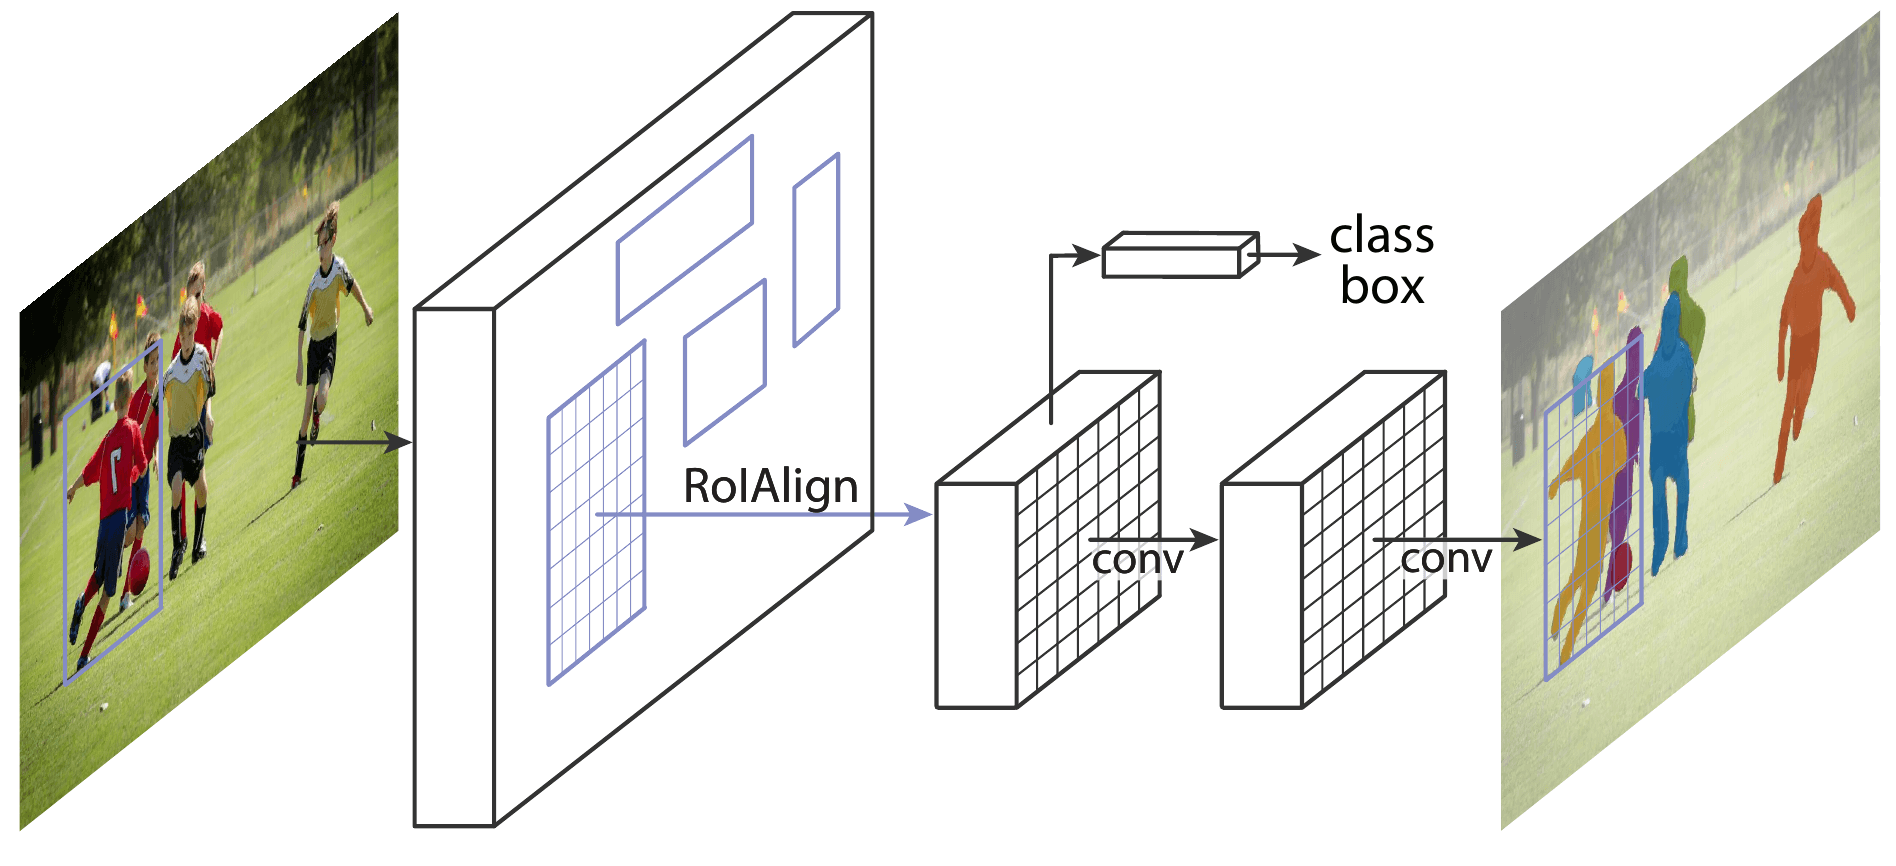
\includegraphics[width=.7\linewidth]{mask_rcnn.png}
	\caption[Mask \acrshort{rcnn} framework]{The Mask \acrshort{rcnn} framework \cite{He2017}. It also generates a segmentation mask in addition to the bounding box and class label.}
	\label{fig:mask_rcnn}
\end{figure}



\section{\glsentryfull{ros}}
\label{sec:ros}
\acrfull{ros} is a framework that allows the communication between sensors and actuators of a robot and is typically run on Linux.
It is a meta-operating system and provides services such as hardware abstraction and low-level device control.
Different languages such as C++, Python or Lisp are supported.
The fundamental concepts are nodes, messages, topics and services \cite{Quigley2009}.
A node is a process that performs computation and should be responsible for only one task.
A package can contain multiple nodes, which can interact with each other.
The communication between nodes is done using messages.
There are different type of messages, but they all consist of standard types such as integer, float or bool, but can also contain other messages.
The messages are published on a specific topic.
The topic can then be subscribed by other nodes, to retrieve the messages.
Services allow for a synchronized communication, instead of the broadcast type topics.\\
A typical communication setup between two nodes can be seen in \cref{fig:ros_framework}.
Node 1 publishes data, e.g. the position of a robot, on a topic.
Node 2 listens to the published data and can then process it.
All the communication is running through the \gls{ros} master.
\begin{figure}[htb]
	\centering
	\documentclass[11pt]{standalone}
\usepackage{tikz}
\usetikzlibrary{shapes.geometric}

\usetikzlibrary{calc, positioning}

\begin{document}
% Define styles
\tikzstyle{block} = [draw, minimum width=2cm, minimum height=1.2cm]

\begin{tikzpicture}
    % Master
    \node [circle, draw] (m) at (0,3) {ROS Master};
    % Nodes
    \node [ellipse, draw, fill=white, minimum width=1cm, minimum height=1cm] (n1) at (-5,0) {Node 1};
    \node [ellipse, draw, fill=white, minimum width=1cm, minimum height=1cm] (n2) at (5,0) {Node 2};
    % Topic
    \node [block] (tp1) at ($(n1)!0.5!(n2)$) {Topic};

    % Connections
    \draw [-stealth] (n1) -- (tp1) node[midway, above] {Publish};
    \draw [-stealth] (tp1) -- (n2) node[midway, above] {Callback};
    \path [-stealth] (n1) edge [bend left] node [left=0.1cm] {Advertising} (m);
    \path [-stealth] (n2) edge [bend right] node [right=0.1cm] {Subscribing} (m);
\end{tikzpicture}
\end{document}
	\caption[\acrshort{ros} communication]{\acrshort{ros} communication between two nodes.}
	\label{fig:ros_framework}
\end{figure}